\externaldocument{Preprocessing.tex}
\chapter{Features}
\label{sec:Features}
In machine learning features are needed for training. What features that are chosen are one of the most critical aspects for a good classifier.
 
\section{Features used to detect barcodes}
\label{sec:Features used to detect barcodes}
Several different features have been tried out but some of them did not given any satisfying result or very similar result. Here are the features presented which are used in the classifiers later on. Some other features are also presented at the end of the chapter. 
\subsection{Standard deviation}
\label{sec:Standard deviation}
One good method to exclude tiles that don't contain any code is to compute the standard deviation of each tile. Tiles which contain code will have a high standard deviation; hence all data with standard deviation under a certain threshold can be discarded. This is a fast method to reduce the amount of data before applying other more complicated features. The standard deviation is calculated according to equation \ref{eq:std}, where $x_i$ are the pixel values in the tile, $N$ is the number of pixels and $\bar{x}$ is the mean.

\begin{equation}
	std = \sqrt{\frac{1}{N}\sum_{i=1}^{N} (x_i-\bar{x})^2}
\end{equation}
\label{eq:std}

\subsection{Structure tensor}
\label{sec:Structure tensor}
The structure tensor, described in \citep{Bigun:1987}, is an effective way to detect 1D-codes and to distinguish between 1D- and 2D-codes, this is illustrated in section \ref{sec:Code detection with AdaBoost}. The structure tensor for a tile is produced by first computing the gradients, this can be done by convolving the tile with a sobel filter. 

\begin{equation}
	\nabla f(x) = \begin{pmatrix} 
		f*g_x \\ f*g_y
	\end{pmatrix}(x)
\end{equation}

The structure tensor is then calculated in the following way:

\begin{equation}	
	T = \int w_2(x) [\nabla_{w_1} f](x)[\nabla_{w_1}^T f](x)\, \mathrm{d}x
\end{equation}

Here $w_1$ and $w_2$ are optional weight functions which typically are Gaussian. The structure tensor will be a 2x2 symmetric matrix:

\begin{equation}
	T = \begin{pmatrix}
			T_{11} & T_{12} \\ T_{21} & T_{22}
		\end{pmatrix}
\end{equation}

The structure tensor can be obtain from the eigenvalues and the normalized eigenvectors:
\begin{equation}
	T = \lambda_1 \hat{e_1}\hat{e_1}^T + \lambda_2 \hat{e_2}\hat{e_2}^T
\end{equation}
The structure tensor can be used in several ways to estimate the structure inside the tile. Areas that contain 1D-codes will have a one dimensional structure, i.e. the gradient in this area will only vary in one direction. On the other hand, areas that contain 2D-codes the variation will be fairly equal in both directions. The amount of variation of the gradient is measured by studying the eigenvalues of the structure tensor.

The following features are calculated for each tile:

\begin{equation}
f_1 = \frac{(\lambda_1 - \lambda_2)^2}{\lambda_1^2+\lambda_2^2}
\end{equation}

\begin{equation}
f_2 = \frac{2\lambda_1\lambda_2}{\lambda_1^2+\lambda_2^2}
\end{equation}

For an area which only varies in one direction the first eigenvalue will be much larger than the second, i.e $f_1$ is close to 1 and $f_2$ is close to 0. For areas which have variation in many directions the values of the two eigenvalues will be more equal, consequently $f_1$ is close to 0 and $f_2$ is close to 1. 

\subsection{FAST corner detection}
\label{sec:FAST corner detection}
FAST (Features from Accelerated Segment Test) is described in \citep{Rosten:2006} and \citep{Rosten:2005}. This is a method to detect corners in images, which is a good way to distinguish between 1D- and 2D-codes, this is illustrated in section \ref{sec:Code detection with AdaBoost}. For a pixel \textit{p} with intensity \textit{I}, consider a circle of 16 pixel and a threshold \textit{t}. The pixel is considered to be a corner if there exist a set of n contiguous pixels in the circle which are all brighter than \textit{I+t} or darker than \textit{I-t}. The algorithm is described in \ref{FAST}.

\begin{figure}[H]
\centering
	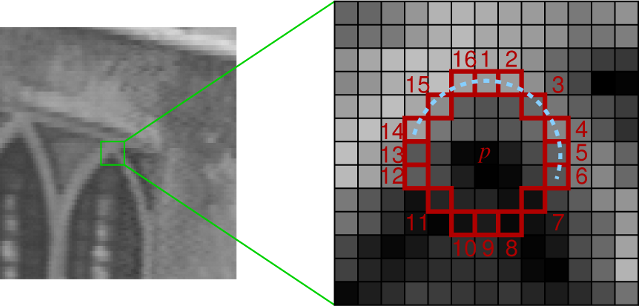
\includegraphics[scale=0.5]{FAST}
	\caption{Image describing FAST corner detection}
	\label{FAST}
\end{figure}

\subsection{Distance map}
\label{sec:Distance map}
A method for barcode detections using a distance map is described in \citep{Bodnar}. The objective of this method is to first calculate the edges in the image by using the canny edge detection algorithm. After that a distance transform is used which in each pixel calculates the closest distance to an edge. There after the mean and standard deviation for the distance map are calculated which are then used as features. The distance map has in this system been used only for detection of 1D-codes.
 
\subsection{Local binary pattern}
\label{sec:Local binary pattern}
Local binary pattern, which is described in \citep{Pietikainen:2010}, is a method that can be used for detection of 2D-codes. The basic idea is to compute a binary code for every pixel, based on the difference of the intensity between the pixel and the surrounding pixels, illustrated in \ref{LBP}. The binary code will then be transformed to a decimal scalar value. If a 3x3 neighbourhood is used there will be 256 different possible values. For each block a histogram will be calculated for all these values. Every bin in the histogram will then be used as a feature. If there is a bin for every possible value, there will be 256 features.

\begin{figure}[H]
\centering
	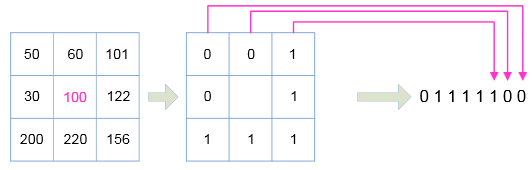
\includegraphics[scale=0.5]{LBP}
	\caption{Image describing local binary pattern}
	\label{LBP}
\end{figure}

\section{Features used for OCR}
\label{sec:Features used for OCR}
Here are the features that have been used for character detection.

\subsection{Two-rectangles}
\label{sec:Two-rectangles}
The two-rectangle features are based on the same idea as the Haar-features presented in \citep{Viola:2010}. This method was used in an earlier project regarding OCR at SICKIVP and showed a rather good result. For that reason it has been tried out in this project as well. The main concept is to use a large number of filters in different sizes consisting of two areas. The result from the filters will then be the difference of the sum of the pixel values between the two areas. There are 17 different filters illustrated in \ref{Two-rectangle} each in different sizes. The sizes of the filters can vary depending how many features that is desired. For example the sizes could be in the range:
\begin{center}
	12x12, 12x16, 16x12, 16x16, 16x20, 20x16, 20x20......40x40
\end{center}
The filters can also have different positions which depends on the size of the tile that is used. For example if the tile has the size 120x120 a filter with the size 12x12 can have totally 100 positions without overlapping each other. If even more features are desired it is also possible to overlap the filters.  
\begin{figure}[H]
\centering
	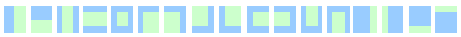
\includegraphics[scale=1]{rectfeatures}
	\caption{Image describing different types of two rectangle features}
	\label{Two-rectangle}
\end{figure}

To make the calculation of the rectangle features faster a s.k. integral image is used. This is a method presented in \citep{Viola:2010} for calculation of Haar-features. An integral image has the same size as the original image. The value for a pixel in the integral image is the sum of all the pixels above and to the left in the original image. If the $i(x,y)$ is the original image the integral image $ii(x,y)$ will be the following.

\begin{equation}
	ii(x,y) = \sum_{x' <= x, y' <= y} i(x',y')
\end{equation}

\subsection{Random point pairs}
\label{sec:Random point pairs}
One type of feature that has been tried out for OCR is a method presented in \citep{Nenad}. The idea is to compare a large amount of point pairs in a tile. The point pairs are randomly chosen but with some constraint. The first point in each pair is chosen from the central part of the tile and the the second point is chosen from the whole tile. There is also a constraint of the distance between the points in each pair. The reason for this is that the character should be somewhat centralized in the tile. If both points are at the edge of the image or if they are too close to each other there will likely be less information to gain. The same point pairs are used for every tile both during training and testing. For each tile the corresponding pixel values are compared in the following way:

 \begin{equation}
 f_i = \left\{ 
   \begin{array}{l l l}
     1 & \quad I(p_1)<I(p_2)\\
     -1 & \quad I(p_1)>I(p_2)\\
     0 & \quad \text{otherwise}
   \end{array} \right.
 \end{equation}
 
Each point pair will then correspond to a feature which can have one of three different values. 
\begin{figure}[H]
\centering
	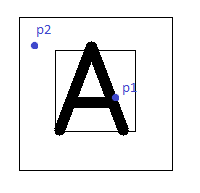
\includegraphics[scale=1]{PointPairs}
	\caption{Image describing two point pairs in a tile}
	\label{PointPairs}
\end{figure}

\subsection{Pixel sums}
\label{sec:Pixel sums}
When using a binary image a simple thing to use as features are sums of pixels for different parts of the tile. Figure \ref{Pixelsums} illustrates a tile divided into 8x8 blocks. The sum of each block will then be a feature. For detection of characters in an image it is desired to get the character centralized in the tile before making a prediction which character it is. This could be used to separate the background from the characters.  

\begin{figure}[H]
\centering
	
\includegraphics[scale=1]{K}
	\caption{Figure illustrates a binary image divided into 8x8 blocks}
	\label{Pixelsums}
\end{figure}
% Local Variables:
% TeX-master: "main.tex"
% End:

\section{Other features}
\label{sec:Other features}
Here are two different feature presented which where considered but never used.
\subsection{Harris corners}
One other way to measure the amount of corners in a tile instead of using FAST corner detection is to use Harris corners. This method is based on the structure tensor explained in section \ref{sec:Structure tensor}. From the structure tensor the Harris corner detector is calculated in the following way:
\begin{equation}
	f_{harris} = det T - k(tr T)^2
\end{equation}
where $k \approx 0.05$. Harris corner detection and FAST corner detection showed very similar result, for that reason only one was used.

\subsection{Random lines}
One method which is a bit similar to the random point pair feature is to use random lines. The idea is to pick point pairs randomly and then define lines between every pair. Every line will then be a feature with a value which depends on how many black or white areas it covers. The lines in figure \ref{PointPairs} will have values between 1 and 5. This feature could be used both for codes and for OCR.  
\begin{figure}[H]
\centering
	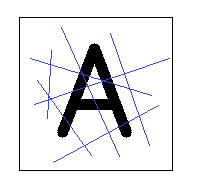
\includegraphics[scale=1]{RandomLines}
	\caption{Image describing some random lines in a tile}
	\label{PointPairs}
\end{figure}
